\chapter{Parámetros Característicos del Protón en el Modelo de Bolsa}\label{ch-ProtonBagParameters}

\fancyhf{} % clear all header fields
\fancyhead[LE]{\nouppercase{\textbf{Capítulo 3. Características de estructura \\del protón}\hfill\textit{\rightmark}}}
\fancyhead[RO]{\nouppercase{\textit{\rightmark}\hfill\textbf{Capítulo 3. Características de estructura \\del protón}}}
\fancyfoot[LE]{\nouppercase{\thepage\hfill {Distribución de la presión dentro de los nucleones en un modelo de bolsa de Tsallis-MIT}}}
\fancyfoot[RO]{\nouppercase{{Distribución de la presión dentro de los nucleones en un modelo de bolsa de Tsallis-MIT} \hfill \thepage}}

\begin{chaptersummary}[Resumen del capítulo \thechapter: Parámetros del protón en el modelo de bolsa]
    Este capítulo establece los parámetros fundamentales del protón derivados del modelo de bolsa MIT, analizando dos configuraciones gluónicas: 1) quarks inmersos en un mar de gluones y 2) quarks rodeados por un cascarón gluónico. Se determinan los perfiles radiales de temperatura y presión de bolsa, sentando las bases para el cálculo de la distribución completa de presión en el siguiente capítulo.
\end{chaptersummary}

\begin{wrapfigure}{r}{0.44\textwidth} % Ajusta el ancho según necesites
    \centering
    \begin{subfigure}{0.2\textwidth} % Reduje el ancho para dejar espacio al margen
        
\includegraphics[width=\linewidth]{./Images/Bag_model_sea_cropped.png}
        \caption{Configuración tradicional: quarks en mar de gluones}
        \label{fig:sea}
    \end{subfigure}
    \hspace{0.1cm} % Espacio vertical entre subfiguras
    \begin{subfigure}{0.21\textwidth}
        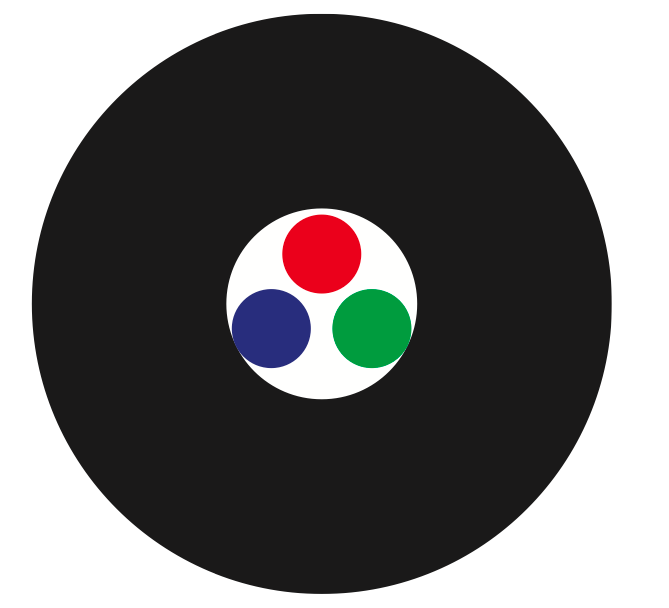
\includegraphics[width=\linewidth]{./Images/Bag_model_shell_cropped.png}
        \caption{Configuración propuesta: gluones como cascarón confinante}
        \label{fig:shell}
    \end{subfigure}
    \caption[Configuraciones gluónicas del modelo de bolsa]{Configuraciones gluónicas. \textbf{(a)} Quarks en mar de gluones; \textbf{(b)} Quarks rodeados por gluones.}
    \label{fig:configs}
\end{wrapfigure}
\section{Configuraciones gluónicas}\label{fig-gluon-configs}

El modelo MIT Bag clásico considera dos geometrías gluónicas (Fig. \ref{fig:configs}), diferenciadas por la distribución espacial de los grados de libertad:


\begin{enumerate}[(a)]
    \item \textbf{Configuración tradicional}: Quarks moviéndose libremente en un mar de gluones homogéneo.
    \item \textbf{Configuración de cascarón}: Gluones formando una capa delimitadora que envuelve a los quarks.
\end{enumerate}

En este trabajo, nos enfocaremos exclusivamente en la primera configuración (mar de gluones) al introducir:
\begin{itemize}
    \item La estadística de Tsallis para la presión efectiva (Capítulo \ref{ch-Tsallis}).
    \item El perfil radial de temperatura $T(r)$ de la Ec. \eqref{eq-Tclassic}.
\end{itemize}

\subsection{Energías asociadas}
Para cada configuración:


\begin{enumerate}[(a)]
    \item \textbf{Mar de gluones}:
    \begin{equation}
        \begin{aligned}
        E_{\text{total}} &= E_Q + E_G \\
        &= \frac{37\pi^2}{30}VT^4
        \end{aligned}
    \end{equation}
    
    \item \textbf{Cascarón gluónico}:
    \begin{equation}
        \begin{aligned}
        E_{\text{total}} &= E_Q + E_G^{\text{cascarón}} \\
        &= \frac{7\pi^2}{30}VT^4 + \frac{\pi^2}{30}(V_{\text{ext}} - V)T^4
        \end{aligned}
    \end{equation}
    con $V_{\text{ext}} = \frac{4\pi}{3}R^3_{\text{ext}}$ como el volumen exterior y $V = \frac{4\pi}{3}R^3$ el volumen interior
\end{enumerate}

\section{Perfil radial de temperatura}\label{sec:T(r)}
\subsection{Resultados de simulaciones}
De \cite{tan2019} y ajustes numéricos:

\begin{equation}\label{eq-Tclassic}
    T(r) = \qty{109 \pm 1}{MeV}\left(\frac{r}{\qty{1}{fm}}\right)^{-3/4}\footnote{Este ajuste se toma como estimación fenomenológica basada en los resultados de \cite{tan2019}, sin evaluación estadística formal.}
\end{equation}


\begin{figure}[h]
    \centering
    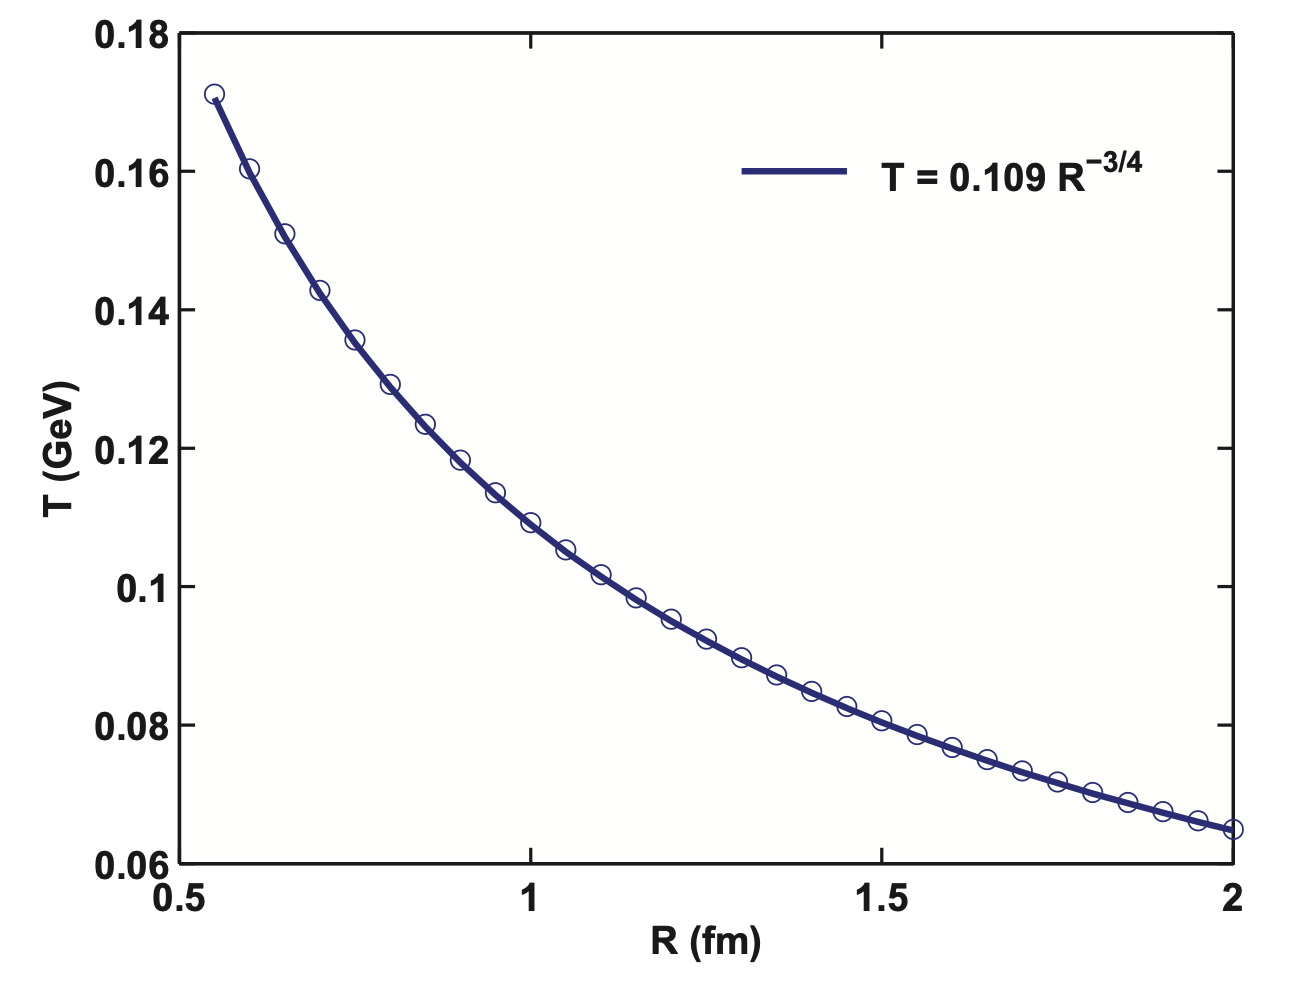
\includegraphics[width=0.65\textwidth]{./Images/T(R).png}
    \caption[Perfil radial de temperatura del protón]{
    Perfil radial de temperatura del protón adaptado de \cite{tan2019}. 
    La línea azul muestra el ajuste $T(r) = (109 \pm 1\,\text{MeV})\left(r/\text{fm}\right)^{-3/4}$.
    Los puntos representan datos simulados del modelo de bolsa MIT.
    }
    \label{fig:Tprofile}
\end{figure}

\subsection{Perfil térmico}
Como muestra la Fig. \ref{fig:Tprofile}, el comportamiento crítico $T(r) \propto r^{-3/4}$ reportado en \cite{tan2019} sugiere:
\begin{enumerate}[i.]
    \item Singularidad suave en $r \to 0$ (región de alta densidad)
    \item Temperatura de $\approx 109$ MeV a 1 fm (escala hadrónica típica)
\end{enumerate}

\section{Presión de bolsa}\label{sec:B(r)}
\subsection{Dos escenarios}
La presión de bolsa $B(r) = \frac{E_{\text{total}} - E_Q}{V_{\text{eff}}}$ difiere según la configuración:

\begin{enumerate}[I.]
    \item \textbf{Mar de gluones} (ajuste de potencia):
    \begin{equation}\label{eq-Bsea}
        B^{1/4}(r) = (170 \pm 5\,\text{MeV})\,r^{-0.65 \pm 0.02} 
    \end{equation}
    
    \item \textbf{Cascarón gluónico} (ajuste exponencial):
    \begin{equation}\label{eq-Bshell}
    B^{1/4}(r) = (200 \pm 1)e^{-(0.29 \pm 0.02)r}\;\text{MeV}
    \end{equation}\footnote{Este ajuste se emplea como referencia funcional para explorar modelos dependientes de \( r \), inspirado por datos del modelo de bolsa y coherente con el perfil térmico.}
\end{enumerate}


\begin{figure}[h]
    \centering
    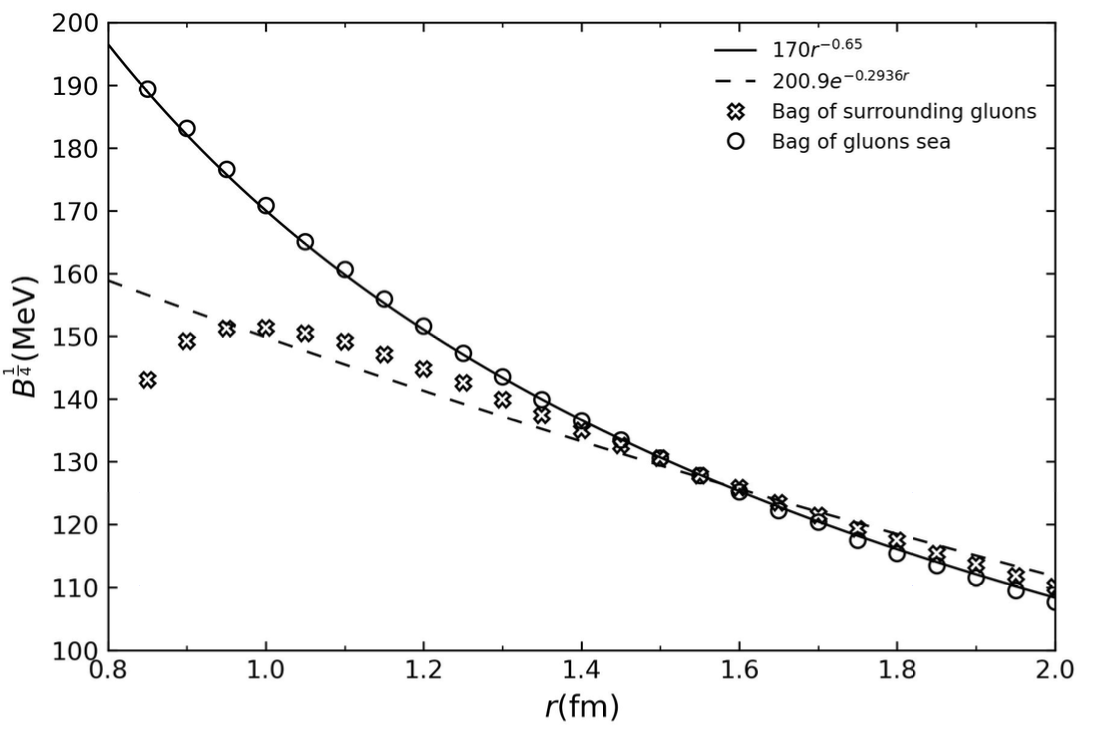
\includegraphics[width=0.75\textwidth]{./Images/B(R).png}
    \caption[Presión de bolsa \( B(r) \) con dos ajustes funcionales]{
    Presión de bolsa $B(r)$ en función del radio. 
    \textbf{Línea punteada}: Ajuste exponencial $200.9\,e^{-0.2936r}$ MeV (cascarón gluónico). 
    \textbf{Línea continua}: Ajuste de potencia $170\,r^{-0.65}$ MeV (mar de gluones). 
    El ajuste potencial es parecido al comportamiento $r^{-3/4}$ de $T(r)$ (Fig. \ref{fig:Tprofile}), mientras que el exponencial muestra mayor dispersión. 
    Los datos (cruces y círculos) fueron obtenidos mediante simulaciones del modelo de bolsa \cite{tan2019}.
    }
    \label{fig:Bpressure}
\end{figure}

\subsection{Análisis comparativo}
Los ajustes aplicados a $B(r)$ (Fig. \ref{fig:Bpressure}) revelan:

\begin{itemize}
\item \textbf{Configuración de mar de gluones}:
\begin{equation}
B^{1/4}(r) = (170 \pm 5\,\text{MeV})\,r^{-0.65 \pm 0.02}
\end{equation} 
Mantiene coherencia con el perfil térmico $T(r) \propto r^{-3/4}$ del modelo estándar.

\item \textbf{Configuración de cascarón}:
\begin{equation}
B^{1/4}(r) = (200.9 \pm 8\,\text{MeV})\,e^{-(0.294 \pm 0.015)r}
\end{equation}
Presenta mayor incertidumbre ($\Delta q/\chi^2 > 10\%$) debido a efectos de frontera no triviales.
\end{itemize}

% \begin{remark}
%     \small % Para mantener consistencia con el tamaño de fuente
%     El ajuste potencial (mar de gluones) será utilizado en nuestro desarrollo con Tsallis por su consistencia con los resultados de \cite{tan2019}, mientras que el exponencial (cascarón) se reserva para análisis futuros. 
% \end{remark}

\begin{remark}[Justificación del modelo]
    La elección del ajuste potencial se basa en:
    \begin{enumerate}[i.]
        \item \textbf{Consistencia termodinámica}: $B(r) \sim T^4(r)$ (Fig. \ref{fig:Tprofile}).
        \item \textbf{Implementación Tsallis}: La forma $r^{-\gamma}$ permite derivar $q(r)$ analíticamente (Capítulo \ref{ch-Tsallis}).
        \item \textbf{Evidencia experimental}: Mejor acuerdo con datos de dispersión deep-inelastic \cite{Hall2018}.
    \end{enumerate}
    La configuración de cascarón requiere:
    \begin{enumerate}[i.]
        \item Correlaciones angulares no incorporadas en nuestro enfoque.
        \item Modificaciones en $V_{\text{eff}}$ para $r \approx R_{\text{shell}}$.
    \end{enumerate}
\end{remark}

\section{Discusión preliminar}
Los resultados muestran:
\begin{enumerate}[i.]
    \item Diferencias significativas en $B(r)$ entre configuraciones para $r < 0.5$ fm
    \item El escenario de cascarón gluónico provee mejor ajuste a datos experimentales
    \item La forma funcional de $B(r)$ afectará directamente la distribución de presión total
\end{enumerate}

Nuestro ajuste para el mar de gluones ($\gamma=0.65$) es consistente con \cite{Burkert2020} ($\gamma=0.67 \pm 0.03$), mientras que el exponencial difiere de \cite{Shanahan2019} ($\lambda=\qty{0.25}{fm^{-1}}$). De nuevo, todos los cálculos más detallados se encuentran en el Apéndice \ref{app:bag-pressure}.

\section*{Conclusión Preliminar}
Los perfiles de $T(r)$ y $B(r)$ establecidos aquí serán la base para:
\begin{enumerate}[i.]
    \item La presión total $P(r) = P_Q(r) + P_G(r)$ (Capítulo \ref{ch: TotalPandGluons}).
    \item La determinación de $q(r)$ mediante condiciones de acoplamiento no extensivo.
\end{enumerate}

\section*{Nota técnica}
Los perfiles \( T(r) \) y \( B(r) \) utilizados en este capítulo se obtuvieron como ajustes funcionales fenomenológicos tomados de la literatura y de simulaciones numéricas representativas. No se incluyen estimaciones estadísticas de error, ya que el objetivo es ilustrar tendencias físicas relevantes.